\documentclass[tikz]{standalone}
\tikzset{circ/.style={circle,draw,inner sep=3pt}}
\begin{document}
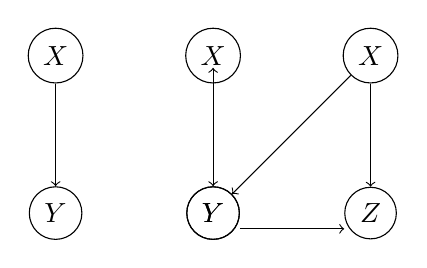
\begin{tikzpicture}[->]
\node[circ] at (-2,0) (x) {$X$};
\node[circ] at (-2,-2) (y) {$Y$};
\path (x) edge (y);
\node[circ] at (0,0) (x') {$X$};
\node[circ] at (0,-2) (y') {$Y$};
\path (x') edge (y');
\path[transform canvas={yshift=2mm}]
  (y') edge (x');
\node[circ] at (2,0) (x'') {$X$};
\node[circ] at (0,-2) (y'') {$Y$};
\node[circ] at (2,-2) (z) {$Z$};
\path (x'') edge (y'');
\path (x'') edge (z);
\path[transform canvas={yshift=-2mm}]
  (y'') edge (z);
\end{tikzpicture}
\end{document}